\documentclass[14pt]{extarticle}
\usepackage[a3paper, landscape, margin=0.8cm, top=0.5cm, bottom=0.5cm]{geometry}
\usepackage{booktabs}
\usepackage{xcolor}
\usepackage{colortbl}
\usepackage{array}
\usepackage{enumitem}
\usepackage{helvet}
\usepackage{graphicx}
\usepackage{tabularx}
\usepackage{adjustbox}
\renewcommand{\familydefault}{\sfdefault}

\definecolor{highlight}{RGB}{0, 102, 204}
\definecolor{rowbg}{RGB}{220, 235, 255}
\definecolor{titlebg}{RGB}{0, 51, 102}
\definecolor{seccolor}{RGB}{0, 102, 204}
\definecolor{secline}{RGB}{0, 102, 204}

\newcommand{\sectionhead}[1]{%
  {\bfseries\color{seccolor}\large #1}\\[-3pt]
  {\color{secline}\rule{\linewidth}{1pt}}\\[1pt]
}

\setlist{noitemsep, topsep=0pt, leftmargin=1.2em}
\pagestyle{empty}
\setlength{\parindent}{0pt}

\begin{document}

%% ── TITLE BAR ───────────────────────────────────────────────────────────────
\colorbox{titlebg}{\parbox{\linewidth}{%
  \centering\color{white}\vspace{1pt}
  {\Large\bfseries Developing an AI Agent to Support Administration and Operation of HPC Systems Based on SLURM}\\[1pt]
  {\small Nguyễn Phúc Thanh Danh \textbf{(2252102)} \quad|\quad HCMUT \quad|\quad Supervisor: Assoc.\ Prof.\ Thoại Nam \quad|\quad Semester 252}
  \vspace{1pt}
}}

%% ── THREE COLUMNS (minipage) ────────────────────────────────────────────────
\noindent
\begin{minipage}[t][26cm][s]{0.30\linewidth}

\sectionhead{Motivation}
\begin{itemize}
  \item Slurm CLI is complex --- dozens of commands, flags, Bash scripting
  \item No safety layer for destructive operations (cancel, hold, release)
  \item Open-weight LLMs lack Slurm tool-calling knowledge
  \item No standardised benchmark for NL-based Slurm agents
\end{itemize}

\vfill
\sectionhead{Approach}
\begin{itemize}
  \item \textbf{Observer/Operator Split:} Read-only Observer + state-changing Operator; destructive actions require human confirmation
  \item \textbf{Grounded RAG:} 273 official Slurm docs $\to$ 2,276 chunks; reduces hallucination
  \item \textbf{Fine-Tuning:} Qwen2.5-14B + QLoRA from GPT-5-mini teacher traces
  \item \textbf{Benchmark:} 3,135 cases, 11 categories, LLM-as-judge scoring
\end{itemize}

\vfill
\sectionhead{Implementation}
\begin{itemize}
  \item \textbf{Stack:} React/Vite $\to$ FastAPI $\to$ MCP $\to$ real Slurm cluster
  \item \textbf{Tools:} 18 typed Slurm tools (\textasciitilde10 Observer, \textasciitilde8 Operator)
  \item \textbf{Training:} 3,329 samples · 3 epochs · A40 48\,GB · QLoRA 4-bit NF4 · \textasciitilde\$20
\end{itemize}

\vfill
\centering
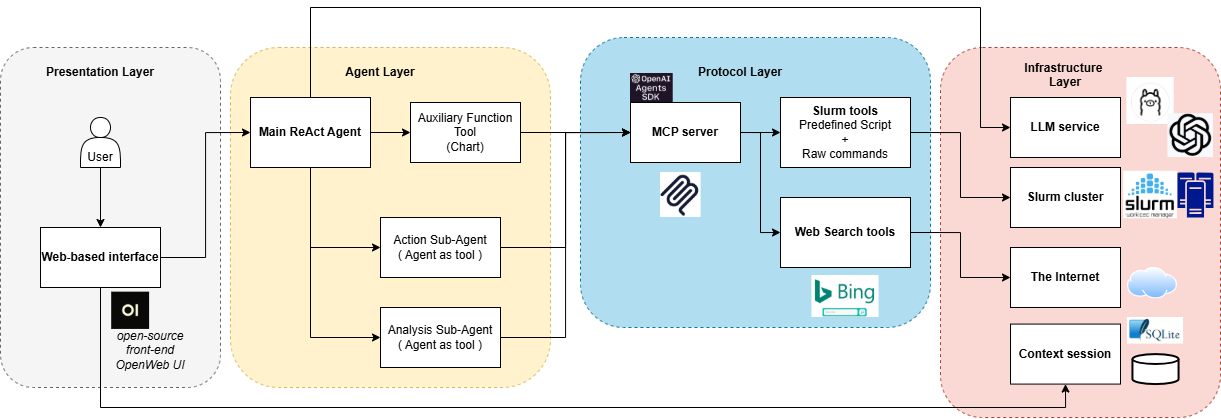
\includegraphics[width=\linewidth, keepaspectratio]{report/images/agent_system_architect.drawio.png}\\[2pt]
{\small\bfseries\color{seccolor} System Architecture}

\end{minipage}%
\hfill
\begin{minipage}[t][26cm][s]{0.38\linewidth}

\sectionhead{Results --- Three-Way Model Comparison}
{\footnotesize 615-case held-out test set (stratified 80/20 split, seed=42)}\\[4pt]
\renewcommand{\arraystretch}{1.3}
\begin{adjustbox}{max width=\linewidth}
\begin{tabular}{lcccccc}
\toprule
\textbf{Model} & \textbf{Pass} & \textbf{Tool} & \textbf{HITL} & \textbf{State} & \textbf{Judge} & \textbf{Lat.} \\
\midrule
GPT-5-mini            & 96.6\% & 98.8\% & 99.0\% & 95.9\% & 74.3\% & 28s \\
\rowcolor{rowbg}
\textbf{\textcolor{highlight}{FT Qwen (ours)}} & \textbf{\textcolor{highlight}{91.4\%}} & \textbf{\textcolor{highlight}{89.2\%}} & \textbf{\textcolor{highlight}{90.4\%}} & \textbf{\textcolor{highlight}{90.0\%}} & \textbf{\textcolor{highlight}{79.7\%}} & \textbf{\textcolor{highlight}{85s}} \\
Base Qwen             & 72.8\% & 84.9\% & 80.8\% & 87.3\% & 76.8\% & 81s \\
Monolithic ablation   & 47.2\% & 77.9\% & 88.9\% & 88.9\% & 59.2\% & 77s \\
\bottomrule
\end{tabular}
\end{adjustbox}

\begin{itemize}
  \item FT model closes \textbf{78\% of the gap} to GPT-5-mini baseline
  \item Observer/Operator beats monolithic by \textbf{+44.2\,pp} pass rate
  \item FT judge (79.7\%) \textbf{exceeds both} base Qwen (76.8\%) and GPT-5-mini (74.3\%)
  \item Tool partitioning cuts selection confusion: docs +41.8\,pp vs.\ monolithic
\end{itemize}

\vfill
\centering
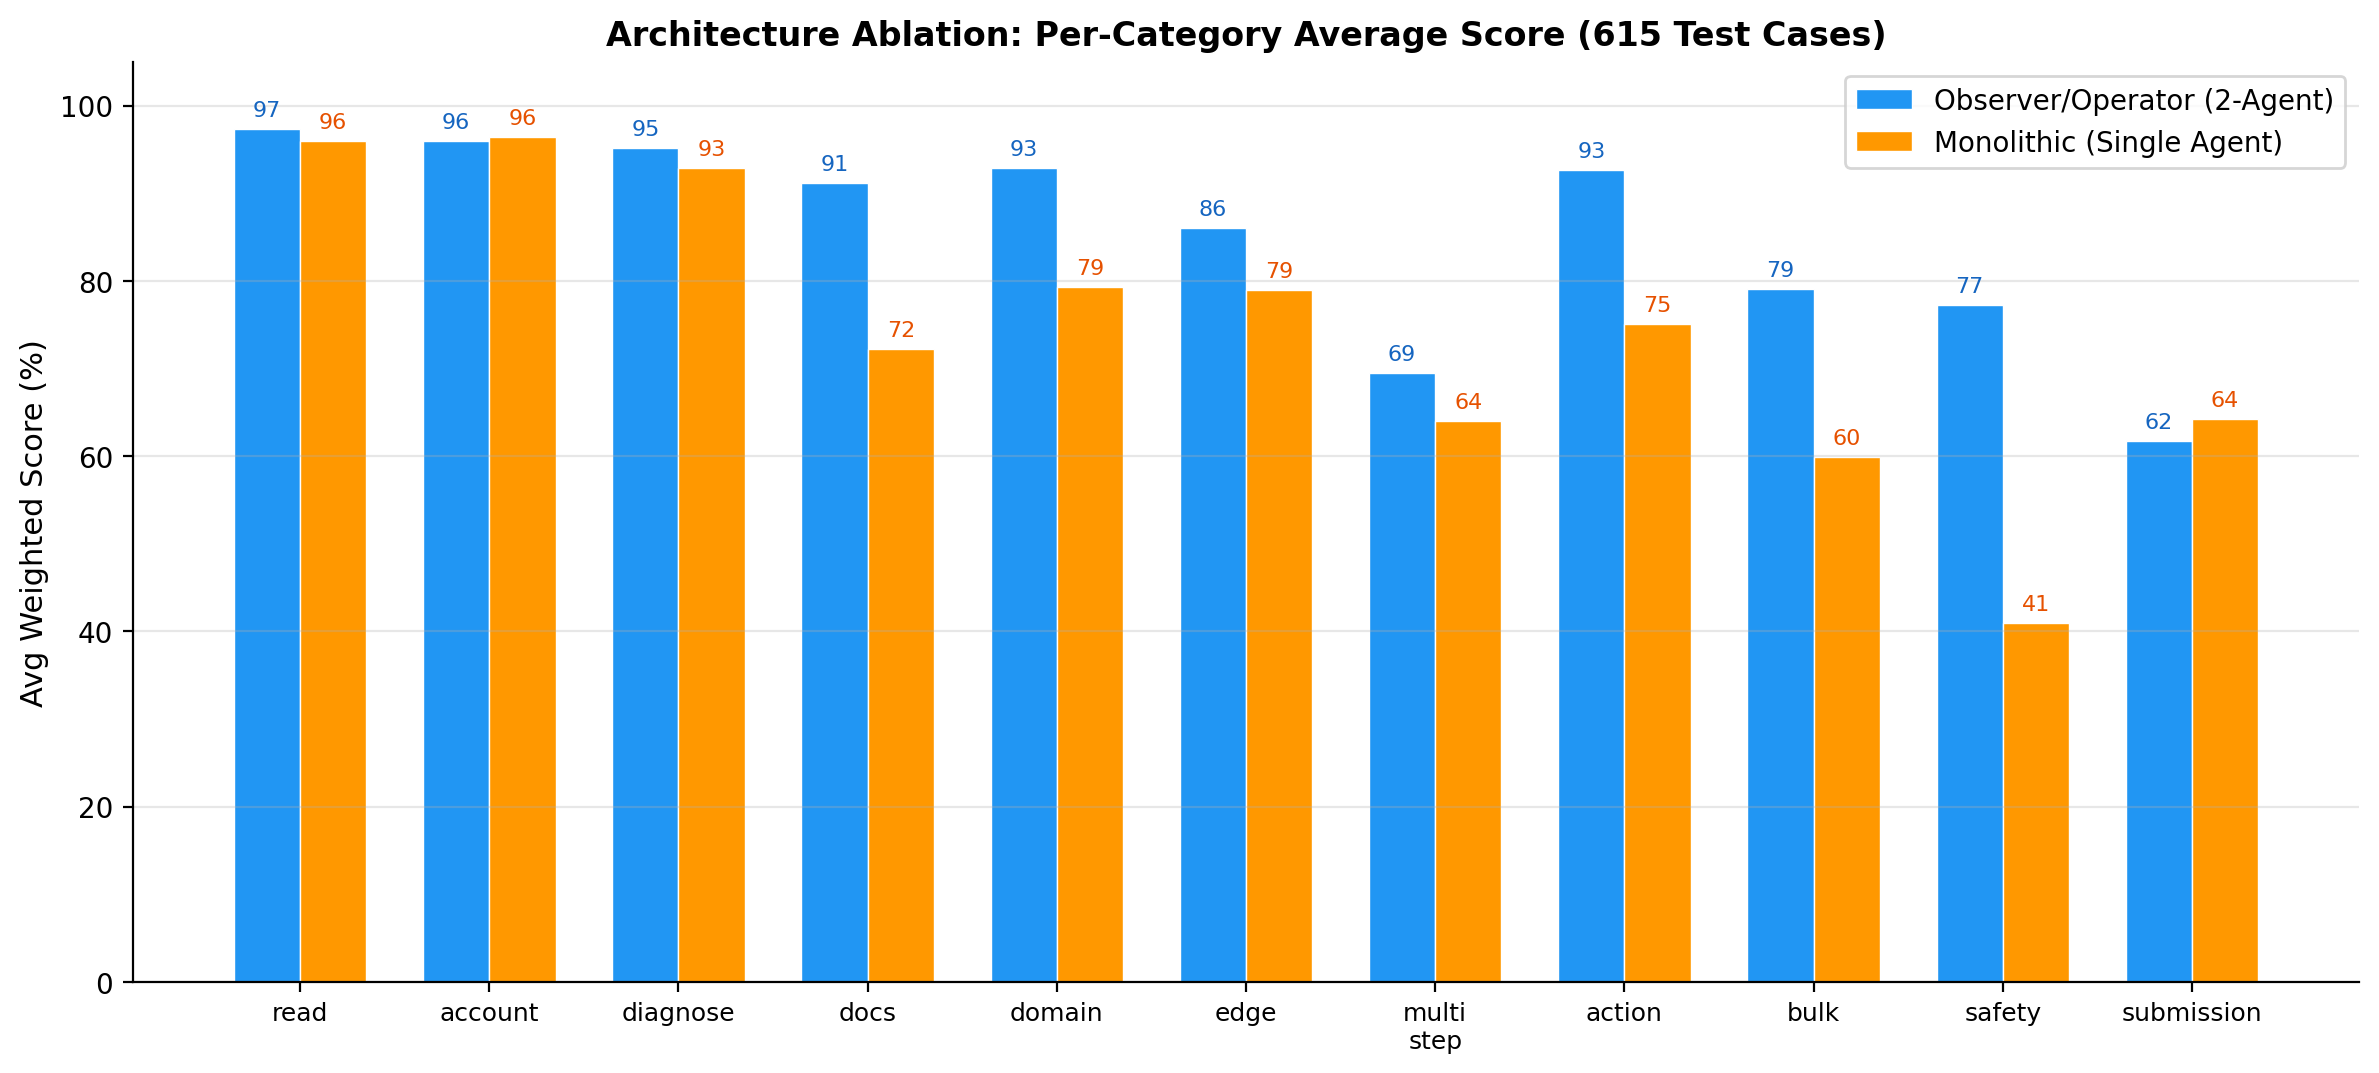
\includegraphics[width=\linewidth, height=7cm, keepaspectratio]{report/images/evaluation/ablation_per_category.png}\\[2pt]
{\small\bfseries\color{seccolor} Per-Category Results (FT vs Base vs Monolithic)}

\vfill
\centering
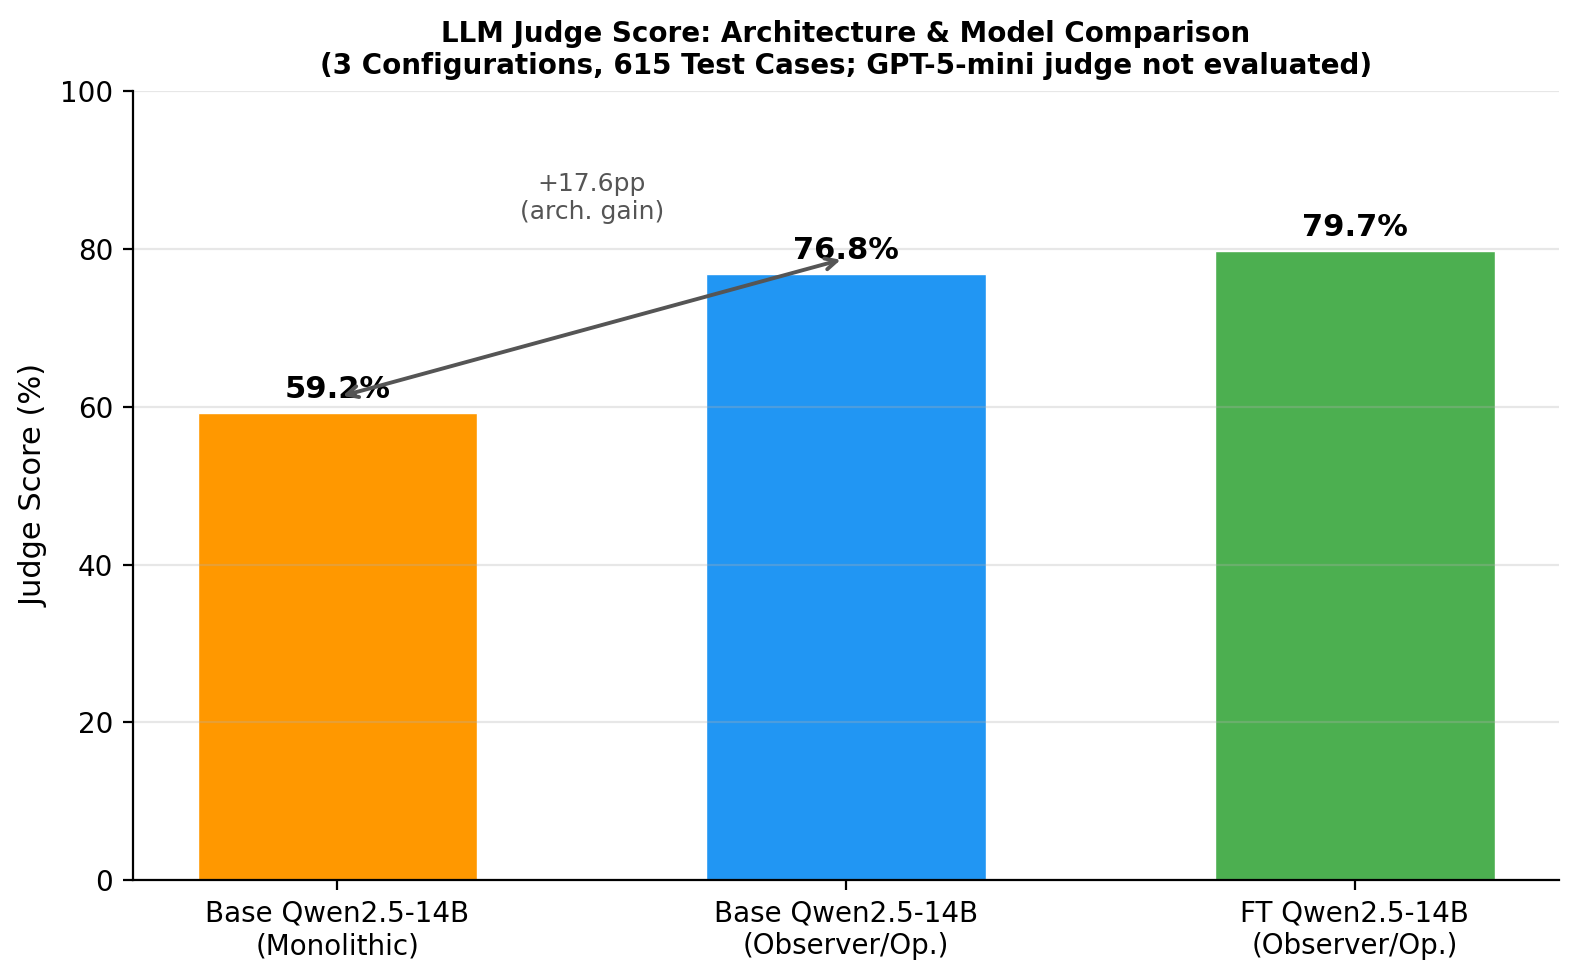
\includegraphics[width=\linewidth, height=7cm, keepaspectratio]{report/images/evaluation/judge_score_comparison.png}\\[2pt]
{\small\bfseries\color{seccolor} LLM Judge Score Comparison}

\end{minipage}%
\hfill
\begin{minipage}[t][26cm][s]{0.28\linewidth}

\sectionhead{Contributions}
\begin{itemize}
  \item Novel \textbf{Observer/Operator} dual-agent safety architecture for Slurm
  \item HITL confirmation workflow for all destructive operations
  \item Grounded RAG pipeline over 273 official Slurm docs
  \item \textbf{3,135-case} curated benchmark with LLM-as-judge scoring
  \item Cost-effective fine-tuning (\textasciitilde\$20) achieving 91.4\% pass rate
\end{itemize}

\vfill
\sectionhead{Future Works}
\begin{itemize}
  \item Multi-tenant authentication, resource isolation, audit logging
  \item Practitioner user studies for usability validation
  \item Expand benchmark to cover more Slurm edge cases
  \item Explore larger open-weight models and multi-turn fine-tuning
\end{itemize}

\vfill
\centering
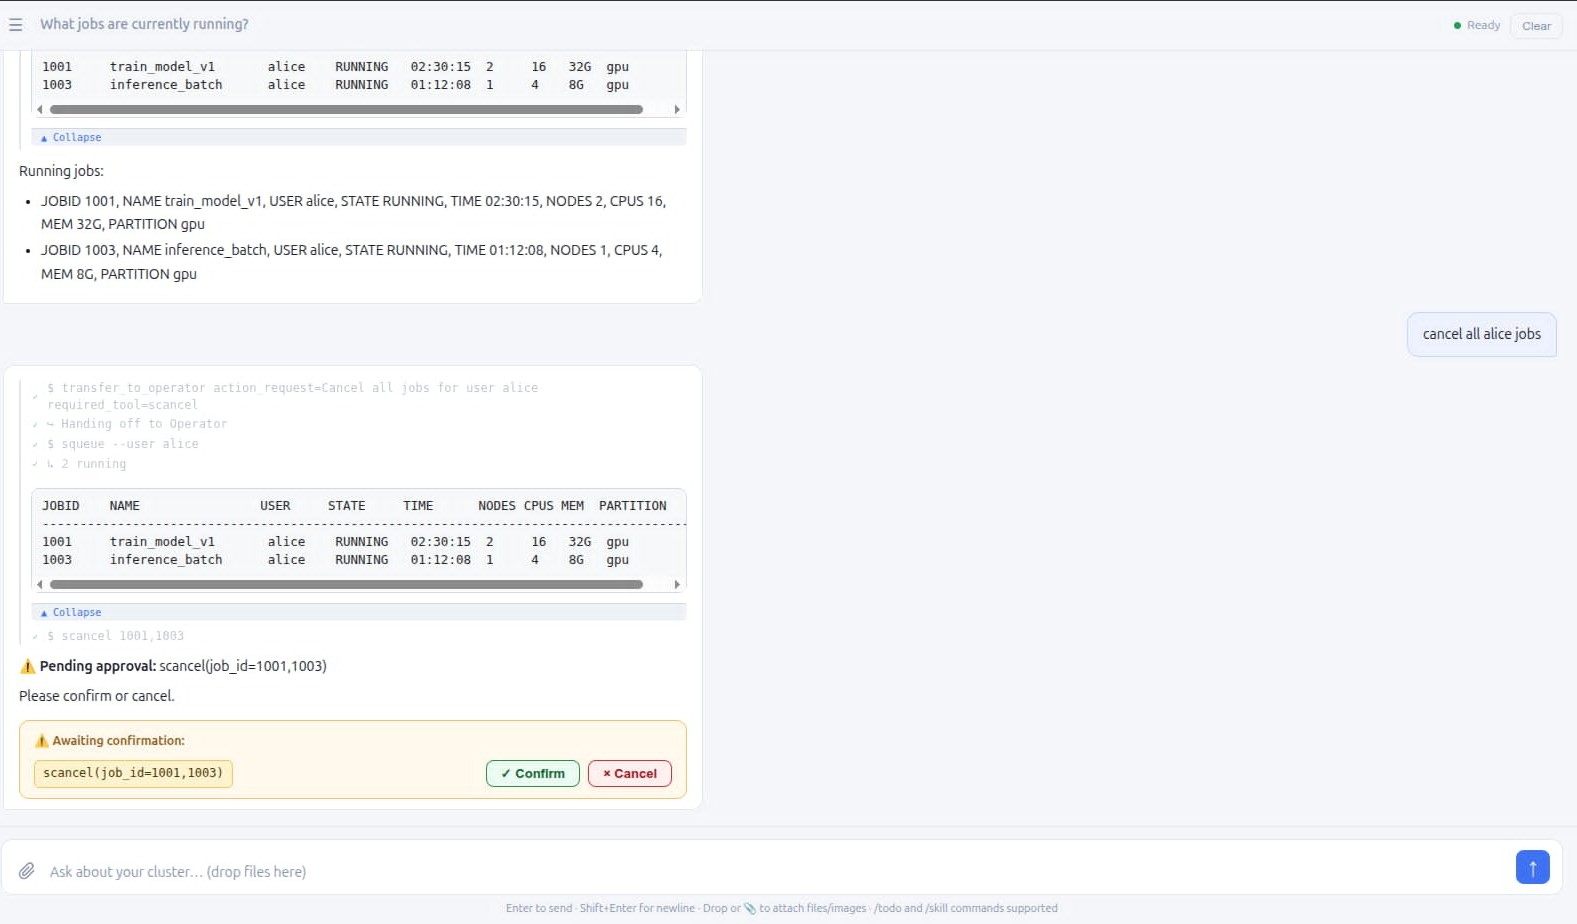
\includegraphics[width=\linewidth, height=5cm, keepaspectratio]{report/images/UI_during_HITL.jpg}\\[2pt]
{\small\bfseries\color{seccolor} HITL Confirmation UI}

\vfill
\centering
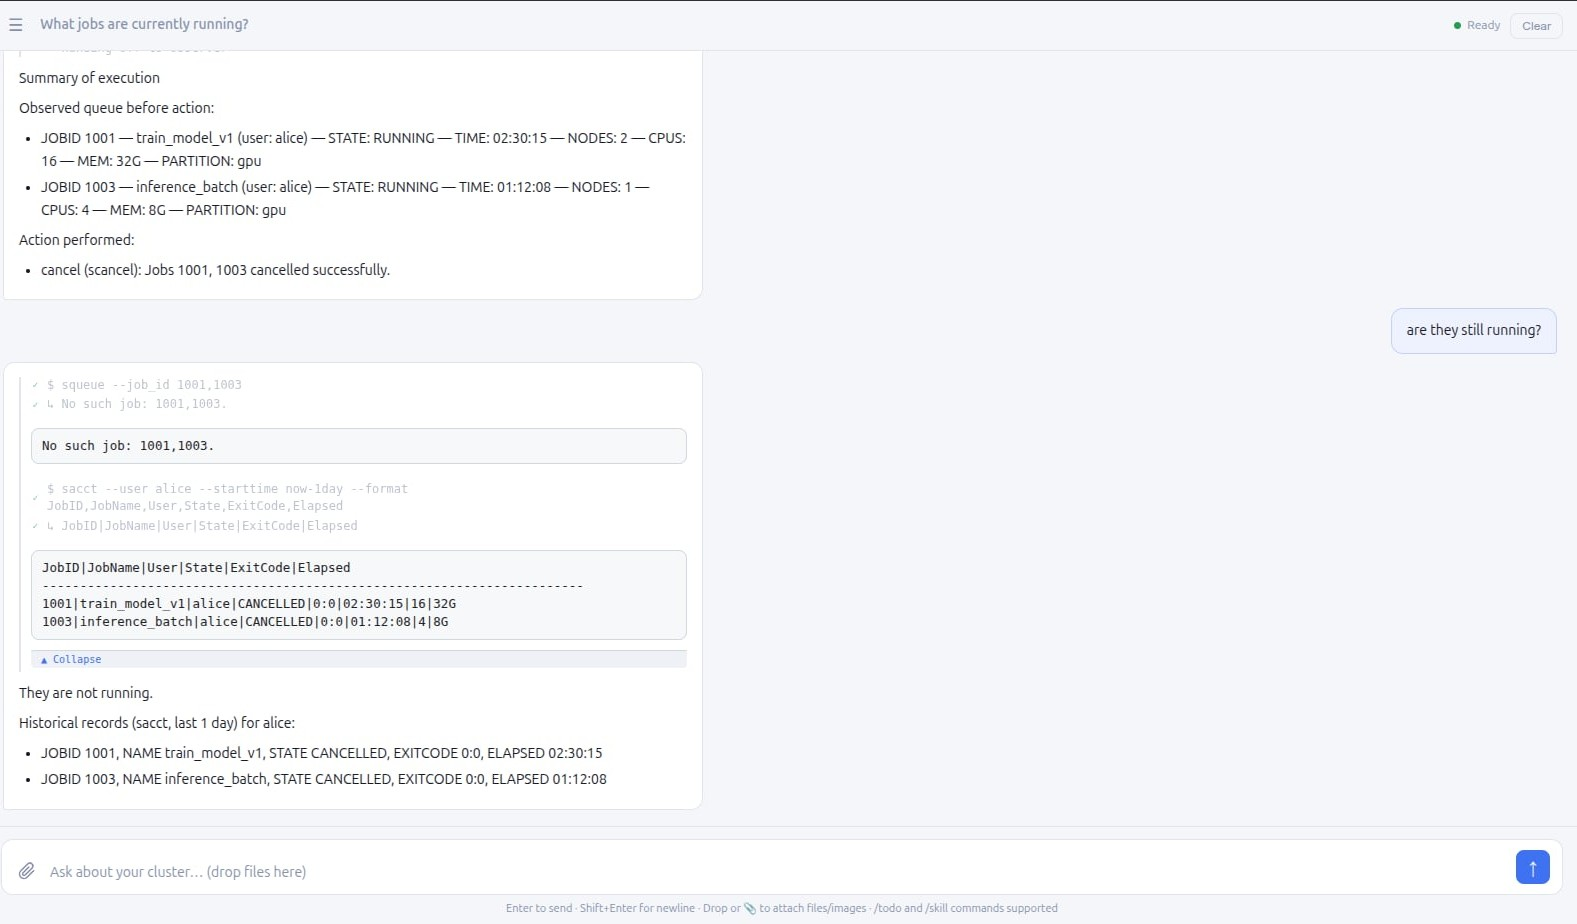
\includegraphics[width=\linewidth, height=5cm, keepaspectratio]{report/images/UI_after_HITL.jpg}\\[2pt]
{\small\bfseries\color{seccolor} UI After HITL Confirmation}

\end{minipage}

\end{document}

\definecolor{highlight}{RGB}{0, 102, 204}
\definecolor{rowbg}{RGB}{220, 235, 255}
\definecolor{titlebg}{RGB}{0, 51, 102}
\definecolor{seccolor}{RGB}{0, 102, 204}

\titleformat{\section}{\large\bfseries\color{seccolor}}{}{0em}{}[\vspace{-4pt}\rule{\linewidth}{1pt}]
\setlength{\columnsep}{1cm}
\setlist{noitemsep, topsep=2pt, leftmargin=1.2em}
\pagestyle{empty}

\begin{document}

%% ── TITLE BAR ──────────────────────────────────────────────────────────────
\colorbox{titlebg}{\parbox{\linewidth}{%
  \centering\color{white}
  \vspace{4pt}
  {\Large\bfseries Developing an AI Agent to Support Administration and Operation of HPC Systems Based on SLURM}\\[2pt]
  {\small Nguyễn Phúc Thanh Danh \quad|\quad HCMUT \quad|\quad Supervisor: Assoc.\ Prof.\ Thoại Nam \quad|\quad Semester 252}
  \vspace{4pt}
}}

\vspace{0.2cm}

%% ── KEY NUMBERS ─────────────────────────────────────────────────────────────
\begin{center}
\renewcommand{\arraystretch}{1.3}
\begin{tabular}{cccc}
  {\LARGE\bfseries\color{highlight} 91.4\%} &
  {\LARGE\bfseries\color{highlight} 78\%} &
  {\LARGE\bfseries\color{highlight} \textasciitilde\$20} &
  {\LARGE\bfseries\color{highlight} 3,135} \\
  FT model pass rate & Gap closed to commercial API & Fine-tuning cost & Benchmark cases \\
\end{tabular}
\end{center}

\vspace{0.15cm}
\begin{multicols}{3}

%% ── COL 1 ───────────────────────────────────────────────────────────────────
\section*{\color{seccolor}Motivation}
\begin{itemize}
  \item Slurm CLI creates barriers for non-expert users
  \item No safety layer for destructive operations (cancel, hold, release)
  \item Open-weight models lack Slurm domain knowledge
  \item No benchmark existed for evaluating NL-based Slurm agents
\end{itemize}

\vspace{0.3cm}
\section*{\color{seccolor}Approach}
\begin{itemize}
  \item \textbf{Observer/Operator Split:} Read-only vs.~state-changing; destructive actions require human confirmation
  \item \textbf{Grounded RAG:} 273 Slurm docs $\to$ 2,276 chunks, local retrieval reduces hallucination
  \item \textbf{Fine-Tuning:} Qwen2.5-14B + QLoRA distilled from GPT-5-mini traces
  \item \textbf{Benchmark:} 3,135 cases across 11 categories, LLM-as-judge scoring
\end{itemize}

\vspace{0.15cm}
\section*{\color{seccolor}Implementation}
\begin{itemize}
  \item \textbf{Stack:} React/Vite $\to$ FastAPI $\to$ MCP tool layer $\to$ Slurm
  \item \textbf{Tools:} 18 typed Slurm tools (\textasciitilde10 Observer, \textasciitilde8 Operator)
  \item \textbf{Training:} 3,329 samples · 3 epochs · A40 48GB GPU · \textasciitilde\$20
\end{itemize}

\columnbreak

%% ── COL 2 ───────────────────────────────────────────────────────────────────
\section*{\color{seccolor}Results — Three-Way Model Comparison (615-case held-out)}
\renewcommand{\arraystretch}{1.3}
\begin{tabular}{lcccccc}
\toprule
\textbf{Model} & \textbf{Pass} & \textbf{Tool} & \textbf{HITL} & \textbf{State} & \textbf{Judge} & \textbf{Latency} \\
\midrule
GPT-5-mini        & 96.6\% & 98.8\% & 99.0\% & 95.9\% & 74.3\%$^\dagger$ & 28.3s \\
\rowcolor{rowbg}
\textbf{\textcolor{highlight}{FT Qwen (ours)}}  & \textbf{\textcolor{highlight}{91.4\%}} & \textbf{\textcolor{highlight}{89.2\%}} & \textbf{\textcolor{highlight}{90.4\%}} & \textbf{\textcolor{highlight}{90.0\%}} & \textbf{\textcolor{highlight}{79.7\%}} & \textbf{\textcolor{highlight}{84.8s}} \\
Base Qwen         & 72.8\% & 84.9\% & 80.8\% & 87.3\% & 76.8\% & 80.9s \\
Monolithic        & 47.2\% & ---    & ---    & ---    & 59.2\% & --- \\
\bottomrule
\multicolumn{7}{l}{\tiny $^\dagger$ Judge score from full 3,135-case baseline run.}
\end{tabular}

\vspace{0.1cm}
\begin{itemize}
  \item FT model closes \textbf{78\% of the gap} to the commercial API baseline
  \item Observer/Operator split beats monolithic by \textbf{+44.2pp pass rate}
  \item FT judge score (79.7\%) \textbf{exceeds both} base (76.8\%) and commercial (74.3\%)
\end{itemize}

\columnbreak

%% ── COL 3 ───────────────────────────────────────────────────────────────────
\section*{\color{seccolor}Contributions}
\begin{itemize}
  \item Observer/Operator safety workflow with HITL confirmation
  \item Grounded RAG layer over 273 official Slurm documentation pages
  \item 3,135-case curated benchmark across 11 categories
  \item Cost-effective open-weight fine-tuning (\textasciitilde\$20, 91.4\% pass rate)
  \item Trace-oriented evaluation stack with LLM-as-judge scoring
\end{itemize}

\vspace{0.15cm}
\section*{\color{seccolor}Future Works}
\begin{itemize}
  \item Multi-tenant auth, tenant isolation, and audit logging
  \item Practitioner user studies for real-world validation
  \item Expand benchmark to more Slurm edge cases
  \item Explore larger open-weight models to close remaining gap
\end{itemize}

\end{multicols}

\end{document}
